\documentclass[12pt,a4paper]{article}
\usepackage[utf8]{inputenc}
\usepackage{amsmath, amssymb}
\usepackage{graphicx}
\usepackage{geometry}
\usepackage{float}
\usepackage{booktabs}
\usepackage{circuitikz}
\usepackage{caption}
\geometry{a4paper, margin=1in}

\title{\textbf{10. Digital electronics}}
\author{Yamulapalli Nandu Navadeep \\ Roll Number: IMS24267}
\date{Date of Experiment: 17/08/2026 \\ Date of Submission: \today}

\begin{document}

\maketitle

\section{Aim of the Experiment}
\begin{enumerate}
    \item To verify the truth table of a BCD to Decimal Decoder using IC 7442.
    \item To design and set up a 4-bit R-2R ladder Digital to Analog Converter (DAC) and measure the analog output voltage for different binary inputs.
\end{enumerate}

\section{Theory}
\subsection{BCD to Decimal Decoder}
A BCD (Binary-Coded Decimal) to decimal decoder is a combinational logic circuit that converts a 4-bit BCD input into one of ten possible decimal digits. The IC 7442 is a commonly used BCD to decimal decoder. It accepts four active-high BCD inputs and provides ten active-low mutually exclusive outputs. When a valid BCD code (0000 to 1001) is applied to the inputs, the corresponding output line goes low (logic 0), while all other output lines remain high (logic 1). For invalid BCD inputs (1010 to 1111), all outputs remain high.

\subsection{Digital to Analog Converter (DAC)}
A Digital to Analog Converter (DAC) converts a digital input signal into a corresponding analog output voltage. The R-2R ladder network is a popular DAC architecture that uses resistors of only two values: $R$ and $2R$. This makes it easier to implement accurately since only the ratio of the resistors matters. 
The digital inputs are applied to the $2R$ resistors in the network. The analog output is proportional to the value of the binary input. The magnitude of the output analog voltage for a 4-bit R-2R DAC is given by the general expression:
$$ V_a = V_H (2^{-1}a_1 + 2^{-2}a_2 + 2^{-3}a_3 + 2^{-4}a_4) $$
Where $V_H$ is the voltage at the logic 1 state, and $a_1, a_2, a_3, a_4$ represent the binary states (0 or 1). The output is maximum when all the inputs are at logic high.

\section{Procedure}
\subsection{BCD to Decimal Decoder}
\begin{enumerate}
    \item Connect the IC 7442 on the trainer kit.
    \item Apply $+5\text{ V}$ to $V_{CC}$ (Pin 16) and connect ground to GND (Pin 8).
    \item Apply the 4-bit binary input to pins 15, 14, 13, and 12 corresponding to A, B, C, and D respectively.
    \item Connect the output pins (1 to 7, 9 to 11) to LEDs to observe the logic states.
    \item Feed binary inputs from 0000 to 1111 and verify the active-low output for each valid BCD input. Observe that all outputs are high for invalid BCD inputs.
\end{enumerate}

\subsection{4-bit R-2R Ladder DAC}
\begin{enumerate}
    \item Set up the R-2R ladder network using $10\text{ k}\Omega$ and $22\text{ k}\Omega$ resistors with an operational amplifier (IC 741).
    \item Provide the necessary power supply ($+15\text{ V}$ and $-15\text{ V}$) to the IC 741.
    \item Manually feed the 4-bit binary inputs from 0000 through 1111.
    \item Measure the analog output voltage at the op-amp output for each binary input using a multimeter.
    \item Record the measured values in a tabular column.
\end{enumerate}

\section{Circuit Diagrams}
\subsection{BCD to Decimal Decoder (IC 7442)}
\begin{figure}[H]
\centering
\begin{circuitikz}[scale=0.8, transform shape]
    % Draw IC 7442 box as a 16-pin DIP
    \draw (0,0) rectangle (4,8);
    \node at (2,7) {\textbf{IC 7442}};
    \node at (2,4.5) {BCD to};
    \node at (2,4) {Decimal Decoder};
    
    % Notch at the top
    \draw (1.5,8) arc (180:360:0.5);
    
    % Left side pins (1 to 8)
    \foreach \y/\pin/\name in {7.5/1/\overline{0}, 6.5/2/\overline{1}, 5.5/3/\overline{2}, 4.5/4/\overline{3}, 3.5/5/\overline{4}, 2.5/6/\overline{5}, 1.5/7/\overline{6}, 0.5/8/\text{GND}} {
        \draw (0,\y) -- (-1.5,\y) node[left] {$\name$ (Pin \pin)};
    }
    
    % Right side pins (16 down to 9)
    \foreach \y/\pin/\name in {7.5/16/V_{CC}, 6.5/15/A_0, 5.5/14/A_1, 4.5/13/A_2, 3.5/12/A_3, 2.5/11/\overline{9}, 1.5/10/\overline{8}, 0.5/9/\overline{7}} {
        \draw (4,\y) -- (5.5,\y) node[right] {$\name$ (Pin \pin)};
    }
\end{circuitikz}
\caption{Pin diagram of BCD to Decimal Decoder (IC 7442)}
\end{figure}

\subsection{4-bit R-2R Ladder DAC}
\begin{figure}[H]
\centering
\begin{circuitikz}[scale=0.8, transform shape]
    % R-2R ladder network
    \draw (-2.5,2) node[ground]{} to[R, l=$R_5$ ($10\text{ k}\Omega$)] (0,2) coordinate (N3);
    \draw (N3) to[R, l=$R_4$ ($10\text{ k}\Omega$), *-*] (2.5,2) coordinate (N2);
    \draw (N2) to[R, l=$R_3$ ($10\text{ k}\Omega$), -*] (5,2) coordinate (N1);
    \draw (N1) to[R, l=$R_2$ ($10\text{ k}\Omega$), -*] (7.5,2) coordinate (N0);
    \draw (N0) to[R, l=$R_1$ ($10\text{ k}\Omega$), -*] (10,2) coordinate (InvertingInput);
    
    % Vertical resistors
    \draw (N3) to[R, l=$R_8$ ($22\text{ k}\Omega$)] (0, -0.5) node[ocirc]{} node[below=2pt] {$B_0$ (LSB)};
    \draw (N2) to[R, l=$R_7$ ($22\text{ k}\Omega$)] (2.5, -0.5) node[ocirc]{} node[below=2pt] {$B_1$};
    \draw (N1) to[R, l=$R_{10}$ ($22\text{ k}\Omega$)] (5, -0.5) node[ocirc]{} node[below=2pt] {$B_2$};
    \draw (N0) to[R, l=$R_6$ ($22\text{ k}\Omega$)] (7.5, -0.5) node[ocirc]{} node[below=2pt] {$B_3$ (MSB)};
    
    % Op-Amp
    \draw (InvertingInput) node[op amp, anchor=-] (OA) {IC 741};
    \draw (OA.+) to[short] ++(0,-0.5) node[ground]{};
    \draw (OA.out) to[short, *-o] ++(1,0) node[right] {$V_{out}$};
    
    % Feedback resistor
    \draw (InvertingInput) -- ++(0,1.5) to[R, l=$R_9$ ($22\text{ k}\Omega$)] ++(2.4,0) -| (OA.out);
    
    % Power supplies
    \draw (OA.up) -- ++(0,0.5) node[above] {$+15\text{ V}$ (7)};
    \draw (OA.down) -- ++(0,-0.5) node[below] {$-15\text{ V}$ (4)};
\end{circuitikz}
\caption{Circuit diagram of 4-bit R-2R Ladder DAC}
\end{figure}

\section{Tabular Column}
\subsection{BCD to Decimal Decoder (IC 7442)}
\begin{table}[H]
\centering
\begin{tabular}{|c|c|c|c|c|c|c|c|c|c|c|c|c|c|}
\hline
\multicolumn{4}{|c|}{\textbf{Inputs}} & \multicolumn{10}{c|}{\textbf{Outputs (Active Low)}} \\
\hline
$A_3$ & $A_2$ & $A_1$ & $A_0$ & $Y_0$ & $Y_1$ & $Y_2$ & $Y_3$ & $Y_4$ & $Y_5$ & $Y_6$ & $Y_7$ & $Y_8$ & $Y_9$ \\
\hline
0 & 0 & 0 & 0 & 0 & 1 & 1 & 1 & 1 & 1 & 1 & 1 & 1 & 1 \\
0 & 0 & 0 & 1 & 1 & 0 & 1 & 1 & 1 & 1 & 1 & 1 & 1 & 1 \\
0 & 0 & 1 & 0 & 1 & 1 & 0 & 1 & 1 & 1 & 1 & 1 & 1 & 1 \\
0 & 0 & 1 & 1 & 1 & 1 & 1 & 0 & 1 & 1 & 1 & 1 & 1 & 1 \\
0 & 1 & 0 & 0 & 1 & 1 & 1 & 1 & 0 & 1 & 1 & 1 & 1 & 1 \\
0 & 1 & 0 & 1 & 1 & 1 & 1 & 1 & 1 & 0 & 1 & 1 & 1 & 1 \\
0 & 1 & 1 & 0 & 1 & 1 & 1 & 1 & 1 & 1 & 0 & 1 & 1 & 1 \\
0 & 1 & 1 & 1 & 1 & 1 & 1 & 1 & 1 & 1 & 1 & 0 & 1 & 1 \\
1 & 0 & 0 & 0 & 1 & 1 & 1 & 1 & 1 & 1 & 1 & 1 & 0 & 1 \\
1 & 0 & 0 & 1 & 1 & 1 & 1 & 1 & 1 & 1 & 1 & 1 & 1 & 0 \\
\hline
1 & 0 & 1 & 0 & 1 & 1 & 1 & 1 & 1 & 1 & 1 & 1 & 1 & 1 \\
\vdots & \vdots & \vdots & \vdots & \multicolumn{10}{c|}{Invalid BCD inputs (All outputs are High)} \\
1 & 1 & 1 & 1 & 1 & 1 & 1 & 1 & 1 & 1 & 1 & 1 & 1 & 1 \\
\hline
\end{tabular}
\caption{Truth Table for BCD to Decimal Decoder (IC 7442)}
\end{table}

\subsection{4-bit R-2R Ladder DAC}
\begin{table}[H]
\centering
\begin{tabular}{|c|c|c|c|c|c|}
\hline
\multicolumn{4}{|c|}{\textbf{Binary Input}} & \textbf{Decimal} & \textbf{Measured Output} \\
$B_3$ & $B_2$ & $B_1$ & $B_0$ & \textbf{Input} & \textbf{Voltage (V)} \\
\hline
0 & 0 & 0 & 0 & 0 & 0 \\
0 & 0 & 0 & 1 & 1 & 0.245 \\
0 & 0 & 1 & 0 & 2 & 0.580 \\
0 & 0 & 1 & 1 & 3 & 0.834 \\
0 & 1 & 0 & 0 & 4 & 1.225 \\
0 & 1 & 0 & 1 & 5 & 1.466 \\
0 & 1 & 1 & 0 & 6 & 1.815 \\
0 & 1 & 1 & 1 & 7 & 2.056 \\
1 & 0 & 0 & 0 & 8 & 2.386 \\
1 & 0 & 0 & 1 & 9 & 2.627 \\
1 & 0 & 1 & 0 & 10 & 2.988 \\
1 & 0 & 1 & 1 & 11 & 3.216 \\
1 & 1 & 0 & 0 & 12 & 3.607 \\
1 & 1 & 0 & 1 & 13 & 3.848 \\
1 & 1 & 1 & 0 & 14 & 3.857 \\
1 & 1 & 1 & 1 & 15 & 4.20 \\
\hline
\end{tabular}
\caption{Analog Voltage output for corresponding Binary Inputs}
\end{table}

\section{Calculations}
The resolution of the DAC can be estimated by taking the difference in measured output voltage for consecutive binary inputs. 
For a 4-bit DAC, the theoretical step size is given by:
$$ \text{Step Size} = \frac{V_{FS}}{2^n - 1} $$
Where $V_{FS}$ is the full-scale voltage and $n=4$.
From our observations, the full scale voltage is approximately $4.20\text{ V}$.
$$ \text{Step Size} \approx \frac{4.20}{15} = 0.28\text{ V} $$
This theoretical step size is consistent with the voltage increments observed between consecutive digital inputs, taking into account experimental uncertainties due to resistor tolerances.

\section{Results}
The truth table of the BCD to Decimal Decoder (IC 7442) was verified successfully, demonstrating active-low outputs for valid BCD inputs and high logic states for invalid inputs.

The 4-bit R-2R ladder Digital to Analog Converter was successfully set up. The analog output voltages for different binary inputs were measured and recorded. The output voltage increased proportionally with the binary input value.

\section{Discussion}
In this experiment, two fundamental digital electronic circuits were studied. First, the IC 7442 decoder was verified. It effectively converted a 4-bit BCD input into a decimal line by driving a specific output low. The observation that invalid BCD inputs (greater than 9) did not trigger any of the zero-to-nine output lines confirmed the designed behavior of the decoder.

The second part of the experiment involved building a 4-bit DAC using an R-2R ladder network and an operational amplifier. The R-2R ladder configuration proved advantageous as it required only two resistance values ($10\text{ k}\Omega$ and $22\text{ k}\Omega$), making the circuit straightforward to construct. The measured analog voltages showed a proportional relationship with the corresponding binary inputs. However, there were slight deviations from perfectly linear voltage steps. These deviations are primarily due to the tolerance values of the resistors used. For a more precise DAC, precision resistors with tight tolerances are required to minimize conversion errors.

\section{References}
\begin{enumerate}
    \item Lab Manual for Advanced Physics Lab II, IISER TVM.
\end{enumerate}

\section{Lab Notes (Observations)}
The following handwritten notes and observations were recorded during the laboratory session.

\begin{figure}[H]
    \centering
    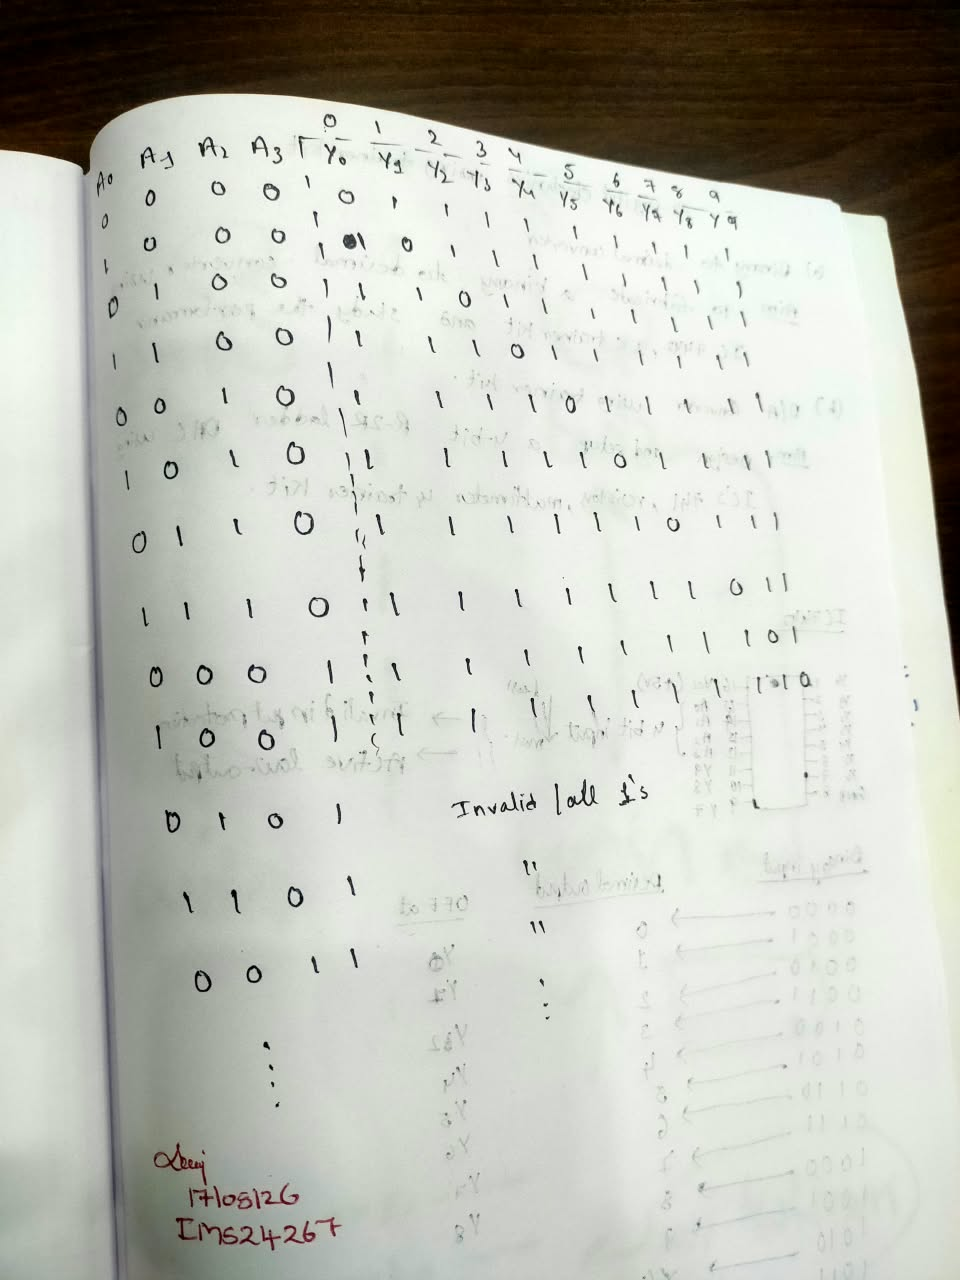
\includegraphics[width=0.85\textwidth]{../Lab observations/Binary to decimal.jpeg}
    \caption{Lab Notes for BCD to Decimal Decoder}
\end{figure}

\begin{figure}[H]
    \centering
    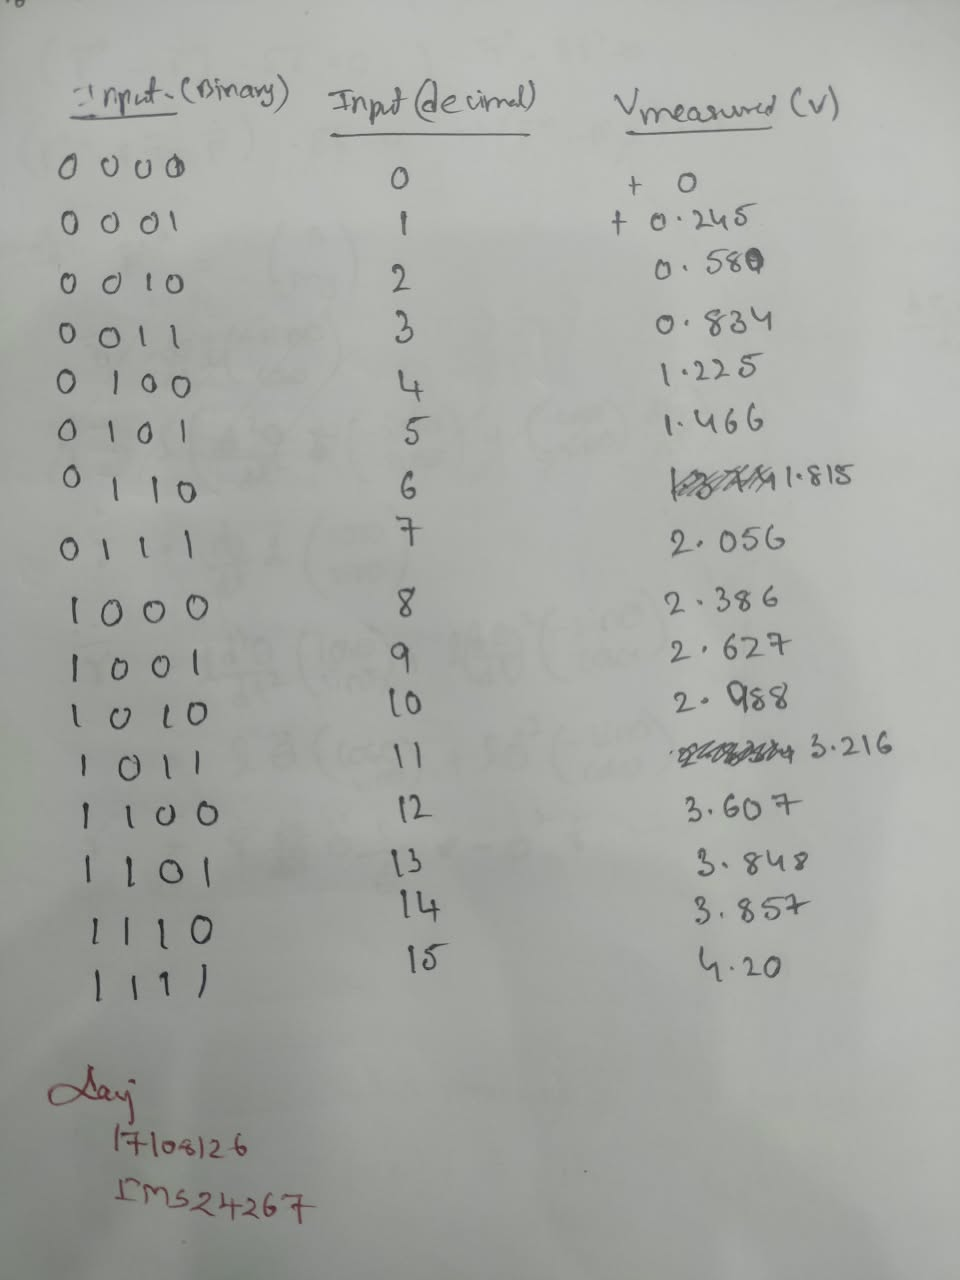
\includegraphics[width=0.85\textwidth]{../Lab observations/Digital to analog.jpeg}
    \caption{Lab Notes for R-2R Digital to Analog Converter}
\end{figure}

\end{document}
